	\section{Data structures}
	The fields and quantities in our PiC model is discretized on a threedimensional grid and comes to use several places in the method. In the multigrid calculation we also have a use for several grids of varying spatial coarseness. So it will be useful for us to organize the data so we have the grid stored as an independent structure available for the program, while the multigrid part uses an extended version where it also has access to the different coarser subgrids. There will also be several types of grid, all with the same specifications, but storing different quantities, so we will use a grid template that all the grids of the same size shares, while we will have a seperate struct containing the quantities in the grid and the specifications.



	\section{Domain partitioning}
		As earlier discussed, in \ref{sec:grid_partitioning} the physical domain covered by our model will be divided onto several processors that each take care of a subdomain. The subdomains are dependent on each other and we need some communication between them, which we solve by letting each subdomain also store the edge of the neighboring subdomain. Depending on the boundary conditions it could also be useful to store an extra set of values on the outer domain boundary as well, which will be called ghost points, \(N_G\). The extra grid points due the the overlap between the subdomains we will call overlap points, \(N_O\). Let us for simplicity sake consider a regular domain, with equal extent in all dimensions, with \(N\) grid points per dimension, \(d\) and consider how many grid values we need to store as a singular domain and the grid values needed when it is divided amongst several processors, a 2 dimensional case is depicted in \cref{fig:domain_part}.

		\subsection{Singular domain}
		In the case where the whole domain is worked on by one process we need \(N^d\) to store the values on the grid representing the physical problem, in addition we see that we also need to store values for the ghost points along the domain boundary. Given that we have one layer of ghost points on all the boundaries, and there is 2 boundaries per dimension, the total number of ghost points is given by \(N_G = 2dN\). Since there is only 1 domain we don't need to account for any overlap between subdomains and the total grid points we need to store is:

		\begin{align}
			N_{Tot} = N^d + N_G + N_O = N^d + 2dN^{d-1}
		\end{align}

		For the 2 dimensional case, in \cref{fig:domain_part}, that adds up to \(N_{Tot} = 8^2 + 2\times4\times 8 = 128\).

		\subsection{Several subdomains}
		In the case where we introduce several subdomain, in addition to storing the grid values and the ghost points we also need to store an overlap between the subdomains. If we take our whole domain \(\Omega\) and divide in up into several small domains \(\Omega_S\), the smaller domains only takes a subsection of the grid points. For simplicity case, and equal load on processors, we let the subdomains as well be regular, with the whole domain being a multiple of the subdomains. Our whole domain has \(N\) grid points in each direction, if we then divide that domain into \(\#\Omega\) domains, then each of those subdomains will have \(N_S = N^d/\#\Omega\) grid points. Each of those subdomains will also need values representing the ghost points and overlap from the neighboring nodes. A boundary of a subdomain will either have overlap points, or ghost points, not both at the same time so for each boundary we need to 1 layer, \( N_S^{d-1}  \). Each subdomain will have \(2\) boundaries per dimension since we have regular subdomains. The total number of grid points needed per subdomain is then

		\begin{align}
			N_{Tot, S} &= N_S^d + (N_G + N_O) =  N_S^d + 2d N_S^{d-1}
			\intertext{while the total number of grid points is}
			N_{Tot} = \#\Omega N_{Tot,S}
		\end{align}

		For the 2 dimensional case discussed earlier we need \( N_{Tot,S} = 4^2 + 2\times2\times4^1 = 32\).

		Since the effect of the subdomain boundaries increase the coarser the grid is we should not let the coarsest multigrid level be to small. We also don't need the spatial extent of the grid to be equal on all sides, but it was done here to keep the computations simple.


	%%%%%%%%%%%%%%%%%%%%%%%%%%%%%%%%%%%%%%%%%%%%%%%%%%%%%%%%%%%%%%%%%%%%%%%%%%%%%%%%%%%%5
	%%%		Tikz picture
	%%%%%%%%%%%%%%%%%%%%%%%%%%%%%%%%%%%%%%%%%%%%%%%%%%%%%%%%%%%%%%%%%%%%%%%%%%%%%%%%%%%%
	\tikzstyle{vertex}=[circle,fill=black!25,minimum size=20pt,inner sep=0pt]
	\tikzstyle{ghost}=[circle,fill=blue!25,minimum size=20pt,inner sep=0pt]
	\tikzstyle{overlap}=[circle,fill=red!50,minimum size=20pt,inner sep=0pt]

	%Note to self: This should really have been done in a more automated/smarter way
	\begin{figure}
		\centering
		\begin{subfigure}[b]{1\textwidth}
		\centering
		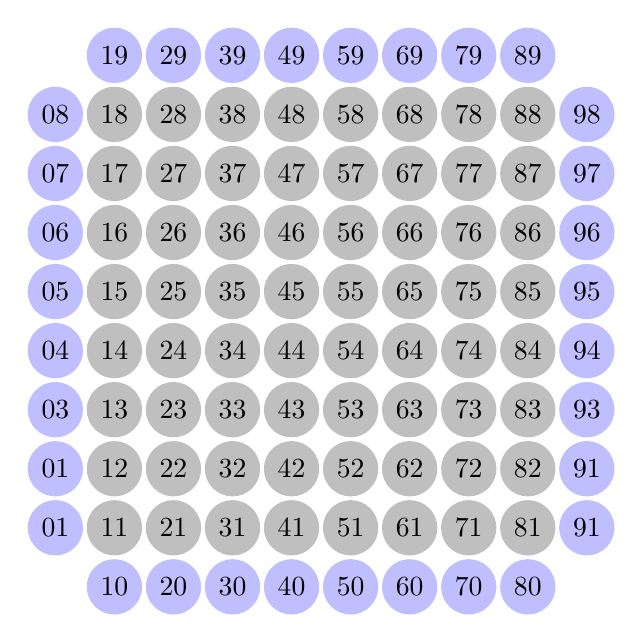
\begin{tikzpicture}[scale=0.75, auto,swap]
	    	%Adding the ghost nodes along the edges
	    	\foreach \pos/\name in 	{				{(1,0)/10}, 	{(2,0)/20},		{(3,0)/30},
	    							 {(4,0)/40},	{(5,0)/50}, 	{(6,0)/60},		{(7,0)/70},
	    							 {(8,0)/80}}
		    \node[ghost] (\name) at \pos {$\name$};
		    \foreach \pos/\name in 	{{(0,1)/01}, 	{(0,2)/01},		{(0,3)/03},
									{(0,4)/04},		{(0,5)/05}, 	{(0,6)/06},		{(0,7)/07},
									{(0,8)/08}}
		    \node[ghost] (\name) at \pos {$\name$};
		    \foreach \pos/\name in 	{	{(1,9)/19}, 	{(2,9)/29},		{(3,9)/39},
	    							 {(4,9)/49},	{(5,9)/59}, 	{(6,9)/69},		{(7,9)/79},
	    							 {(8,9)/89}}
		    \node[ghost] (\name) at \pos {$\name$};
		    \foreach \pos/\name in 	{	{(9,1)/91}, 	{(9,2)/91},		{(9,3)/93},
									{(9,4)/94},		{(9,5)/95}, 	{(9,6)/96},		{(9,7)/97},
									{(9,8)/98}}
		    \node[ghost] (\name) at \pos {$\name$};
		    %The inner nodes
		    \foreach \pos/\name in {{(1,1)/11}, 	{(1,2)/12},		{(1,3)/13},		{(1,4)/14},
		    						{(1,5)/15}, 	{(1,6)/16},		{(1,7)/17},		{(1,8)/18}}
		    \node[vertex] (\name) at \pos {$\name$};
		    \foreach \pos/\name in {{(2,1)/21}, 	{(2,2)/22},		{(2,3)/23},		{(2,4)/24},
		    						{(2,5)/25}, 	{(2,6)/26},		{(2,7)/27},		{(2,8)/28}}
		    \node[vertex] (\name) at \pos {$\name$};
		    \foreach \pos/\name in {{(3,1)/31}, 	{(3,2)/32},		{(3,3)/33},		{(3,4)/34},
		    						{(3,5)/35}, 	{(3,6)/36},		{(3,7)/37},		{(3,8)/38}}
		    \node[vertex] (\name) at \pos {$\name$};
		    \foreach \pos/\name in {{(4,1)/41}, 	{(4,2)/42},		{(4,3)/43},		{(4,4)/44},
		    						{(4,5)/45}, 	{(4,6)/46},		{(4,7)/47},		{(4,8)/48}}
		    \node[vertex] (\name) at \pos {$\name$};
		    \foreach \pos/\name in {{(5,1)/51}, 	{(5,2)/52},		{(5,3)/53},		{(5,4)/54},
		    						{(5,5)/55}, 	{(5,6)/56},		{(5,7)/57},		{(5,8)/58}}
		    \node[vertex] (\name) at \pos {$\name$};
		    \foreach \pos/\name in {{(6,1)/61}, 	{(6,2)/62},		{(6,3)/63},		{(6,4)/64},
		    						{(6,5)/65}, 	{(6,6)/66},		{(6,7)/67},		{(6,8)/68}}
		    \node[vertex] (\name) at \pos {$\name$};
		    \foreach \pos/\name in 	{{(7,1)/71}, 	{(7,2)/72},		{(7,3)/73},		{(7,4)/74},
		    						{(7,5)/75}, 	{(7,6)/76},		{(7,7)/77},		{(7,8)/78}}
		    \node[vertex] (\name) at \pos {$\name$};
		    \foreach \pos/\name in 	{{(8,1)/81}, 	{(8,2)/82},		{(8,3)/83},		{(8,4)/84},
		    						{(8,5)/85}, 	{(8,6)/86},		{(8,7)/87},		{(8,8)/88}}
		    \node[vertex] (\name) at \pos {$\name$};
	    \end{tikzpicture}
	    \caption{The grid points needed for an \(8\cross8\) domain.}
		\end{subfigure}
		\begin{subfigure}[b]{1\textwidth}
		\centering
		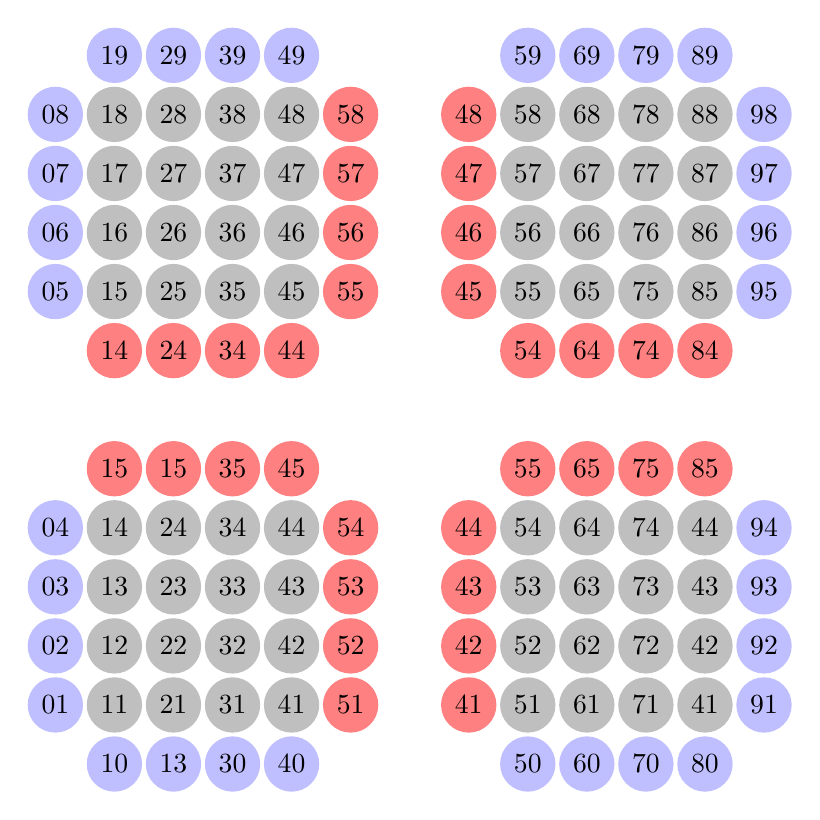
\begin{tikzpicture}[scale=0.75, auto,swap]
	    	%Left bottom corner inner
	    	\foreach \pos/\name in 	{{(1,1)/11}, 	{(1,2)/12},		{(1,3)/13},		{(1,4)/14},
		    						{(2,1)/21}, 	{(2,2)/22},		{(2,3)/23},		{(2,4)/24},
		    						{(3,1)/31}, 	{(3,2)/32},		{(3,3)/33},		{(3,4)/34},
		    						{(4,1)/41}, 	{(4,2)/42},		{(4,3)/43},		{(4,4)/44}}
		    \node[vertex] (\name) at \pos {$\name$};
		    %Left bottom corner outer
		    \foreach \pos/\name in 	%Bottom
		    	{{(1,0)/10},		{(2,0)/13},		{(3,0)/30},		{(4,0)/40}}
		    \node[ghost] (\name) at \pos {$\name$};
		    \foreach \pos/\name in 	%Top
		    	{{(1,5)/15},		{(2,5)/15},		{(3,5)/35},		{(4,5)/45}}
		    \node[overlap] (\name) at \pos {$\name$};
		    \foreach \pos/\name in 	%Left
		    	{{(0,1)/01}, 	{(0,2)/02},		{(0,3)/03},		{(0,4)/04}}
		    \node[ghost] (\name) at \pos {$\name$};
		    \foreach \pos/\name in 	%Right
		    	{{(5,1)/51}, 	{(5,2)/52},		{(5,3)/53},		{(5,4)/54}}
		    \node[overlap] (\name) at \pos {$\name$};
		    %Left bottom corner inner
	    	\foreach \pos/\name in 	{{(8,1)/51}, 	{(8,2)/52},		{(8,3)/53},		{(8,4)/54},
		    						{(9,1)/61}, 	{(9,2)/62},		{(9,3)/63},		{(9,4)/64},
		    						{(10,1)/71}, 	{(10,2)/72},	{(10,3)/73},	{(10,4)/74},
		    						{(11,1)/41}, 	{(11,2)/42},	{(11,3)/43},	{(11,4)/44}}
		    \node[vertex] (\name) at \pos {$\name$};
		    %Right bottom corner outer
		    \foreach \pos/\name in 	%Bottom
		    	{{(8,0)/50},		{(9,0)/60},		{(10,0)/70},		{(11,0)/80}}
		    \node[ghost] (\name) at \pos {$\name$};
		    \foreach \pos/\name in 	%Top
		    	{{(8,5)/55},		{(9,5)/65},		{(10,5)/75},		{(11,5)/85}}
		    \node[overlap] (\name) at \pos {$\name$};
		    \foreach \pos/\name in 	%Left
		    	{{(7,1)/41}, 	{(7,2)/42},		{(7,3)/43},		{(7,4)/44}}
		    \node[overlap] (\name) at \pos {$\name$};
		    \foreach \pos/\name in 	%Right
		    	{{(12,1)/91}, 	{(12,2)/92},	{(12,3)/93},		{(12,4)/94}}
		    \node[ghost] (\name) at \pos {$\name$};
		    %Left top corner inner
	    	\foreach \pos/\name in 	{{(1,8)/15}, 	{(1,9)/16},		{(1,10)/17},		{(1,11)/18},
		    						{(2,8)/25}, 	{(2,9)/26},		{(2,10)/27},		{(2,11)/28},
		    						{(3,8)/35}, 	{(3,9)/36},		{(3,10)/37},		{(3,11)/38},
		    						{(4,8)/45}, 	{(4,9)/46},		{(4,10)/47},		{(4,11)/48}}
		    \node[vertex] (\name) at \pos {$\name$};
		    %Left top corner outer
		    \foreach \pos/\name in 	%Bottom
		    	{{(0,8)/05},	{(0,9)/06},		{(0,10)/07},	{(0,11)/08}}
		    \node[ghost] (\name) at \pos {$\name$};
		    \foreach \pos/\name in 	%Top
		    	{{(5,8)/55},	{(5,9)/56},		{(5,10)/57},	{(5,11)/58}}
		    \node[overlap] (\name) at \pos {$\name$};
		     \foreach \pos/\name in %Left
		    	{{(1,7)/14}, 	{(2,7)/24},		{(3,7)/34},		{(4,7)/44}}
		    \node[overlap] (\name) at \pos {$\name$};
		    \foreach \pos/\name in 	%Right
		    	{{(1,12)/19}, 	{(2,12)/29},	{(3,12)/39},	{(4,12)/49}}
		    \node[ghost] (\name) at \pos {$\name$};
		    %Right top corner inner
	    	\foreach \pos/\name in 	{{(8,8)/55}, 	{(8,9)/56},		{(8,10)/57},		{(8,11)/58},
		    						{(9,8)/65}, 	{(9,9)/66},		{(9,10)/67},		{(9,11)/68},
		    						{(10,8)/75}, 	{(10,9)/76},	{(10,10)/77},		{(10,11)/78},
		    						{(11,8)/85}, 	{(11,9)/86},	{(11,10)/87},		{(11,11)/88}}
		    \node[vertex] (\name) at \pos {$\name$};
		    %Right top corner outer
		    \foreach \pos/\name in 	%Bottom
		    	{{(7,8)/45},	{(7,9)/46},		{(7,10)/47},	{(7,11)/48}}
		    \node[overlap] (\name) at \pos {$\name$};
		    \foreach \pos/\name in 	%Top
		    	{{(12,8)/95},	{(12,9)/96},	{(12,10)/97},	{(12,11)/98}}
		    \node[ghost] (\name) at \pos {$\name$};
		     \foreach \pos/\name in %Left
		    	{{(8,7)/54}, 	{(9,7)/64},		{(10,7)/74},	{(11,7)/84}}
		    \node[overlap] (\name) at \pos {$\name$};
		    \foreach \pos/\name in 	%Right
		    	{{(8,12)/59}, 	{(9,12)/69},	{(10,12)/79},	{(11,12)/89}}
		    \node[ghost] (\name) at \pos {$\name$};
	    \end{tikzpicture}
	    \caption{The \(8\cross8\) grid divided into 4 subdomains}
		\end{subfigure}
		\caption{Each circle in the figures represents 1 grid point, and the first number is the column while the second is the row. The grey colour represents physical space the computational node works on, the blue color is the outer grid points for boundary conditions and the red colour is the overlapping grid points.}
		\label{fig:domain_part}
    \end{figure}
